\documentclass{article}

\usepackage{geometry}
\usepackage{times}
\usepackage{epsfig}
\usepackage{graphicx}
\usepackage{amsmath}
\usepackage{amssymb}
\usepackage{bm}

\setcounter{page}{1}
\setlength{\parindent}{0pt}
\begin{document}

\title{Kernelization on Neural Network}
\author{Shuai Zhang\and Yingchun Zhang}
\maketitle

%-------------------------------------------------------------------------
\section{Introduction}

\subsection{Related Works}
Wilson et al. \cite{DBLP:journals/corr/WilsonHSX15} combined the non-parametric flexibility of kernel methods with the structural properties of deep neural networks.

%\cite{DBLP:conf/aistats/PandeyD14} 



%-------------------------------------------------------------------------
\section{Methods}

\subsection{Neural Network}

In a two-layer network, the feed-forward network function is

\begin{equation}
\mathbf{y}_k(\mathbf{x}, \mathbf{w}) = h^{(2)}\left(\sum_{j=0}^{M}w_{kj}^{(2)}h^{(1)}\left(\sum_{i=0}^{D}w_{ji}^{(1)}x_i\right)\right).
\end{equation}

Given a training set with input vectors $\{\mathbf{x}_n\}$, where $n = 1, ..., N$, together with a correspounding set of target vectors $\{\mathbf{t}_n\}$, we minimize the error function

\begin{equation}
E(\mathbf{w}) = \frac{1}{2} \sum_{n=1}^{N} {\|\mathbf{y}(\mathbf{x}_n, \mathbf{w}) - \mathbf{t}_n\|}^2.
\end{equation}




%-------------------------------------------------------------------------
\subsection{Kernelized Neural Network}

%----------------------------------@ July 24---------------------------------------
\newpage
\par\par\LARGE Progress @ July 24\normalsize

\subsubsection{Nonparametric representation}


\par \textbf{Single-layer neural network}\\

\begin{figure}[h]
\centering
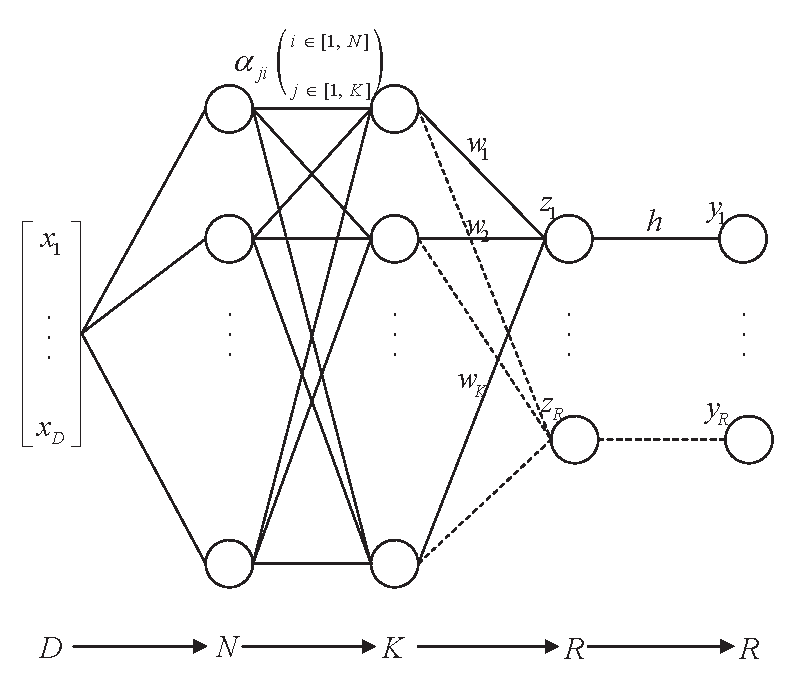
\includegraphics[height=7cm]{Non-para_single-layer}
\end{figure}

\par In a single-layer neural network, the feed-forward network function is 
\begin{equation}
y_n = h \left( \sum\limits_{j=1}^{K} w_{j} \left( \sum\limits_{i=1}^{N} \alpha_{ji} k( \mathbf{x}_{i} , \mathbf{x}_{n}) \right)\right)
\end{equation} 

where $ \{ \mathbf{x}_{i}\}_{i=1}^{N}$ is the unique sample which is a $D$-dimension vector of the dataset, $k$ is a kernel function which builds a new inner product space, and we try to get k linear combination of with the weight $\alpha_{ji}$, then we make a linear combination of the new base with the weight $ w_{j}$. $h$ is an activation function and so as follows.  
All the $w, h, \alpha, k$ and $\mathbf{x}$ shown in the following part have the same meaning as the former ones.\\



\par \textbf{Multi-layer neural network} \\

\begin{figure}[h]
\centering
\includegraphics[height=7cm]{Non-para_muti-layer}
\end{figure}

\begin{equation}
y_n = h^{(2)} \left( \sum\limits_{j=1}^{K} w_{j}^{(2)} \left( \sum\limits_{i=1}^{N} \alpha_{ji}^{(2)} k_2( \mathbf{x}_{i},\left[               
  \begin{array}{c}   
    h^{(1)} \left( \sum\limits_{j=1}^{K} w_{1j}^{(1)} \left( \sum\limits_{i=1}^{N} \alpha_{ji}^{(1)}k_1( \mathbf{x}_{i},\mathbf{x}_n) \right) \right)\\  
    .\\  
    .\\  
    .\\
    h^{(1)} \left( \sum\limits_{j=1}^{K} w_{Mj}^{(1)} \left( \sum\limits_{i=1}^{N} \alpha_{ji}^{(1)}k_1( \mathbf{x}_{i},\mathbf{x}_n) \right) \right)\\
  \end{array}
\right] )
 \right) \right)
\end{equation} 

\par The number in superscript of the symbols represents the layer of neural network, such as, $w_j^{(2)}$ means the weight of the second layer of neural network and so as follows. \\



\subsubsection{Parametric representation}


\par \textbf{Single-layer neural network}\\

\begin{figure}[h]
\centering
\includegraphics[height=7cm]{Para_single-layer}
\end{figure}

\begin{equation}
y_n = h \left( \sum\limits_{j=1}^K w_j k( \bm{\alpha}_j, \mathbf{x}_{n}) \right)
\end{equation}
\par $\bm{\alpha}_j$ is the center of kernel which is a D-dimension vector.\\





\par \textbf{Multi-layer neural network}\\

\begin{figure}[h]
\centering
\includegraphics[height=7cm]{Para_muti-layer}
\end{figure}

\begin{equation}
y_n = h^{(2)} \left( \sum\limits_{j=1}^K w_j^{(2)} k_2( \bm{\alpha}_j^{(2)}, \left[ \begin{array}{c}
	h^{(1)} \left( \sum\limits_{i=1}^K w_{1i}^{(1)} k_1(\bm{\alpha}_i^{(1)},\mathbf{x}_n) \right)\\
	.\\
	.\\
	.\\
	h^{(1)} \left( \sum\limits_{i=1}^K w_{Mi}^{(1)} k_1(\bm{\alpha}_i^{(1)},\mathbf{x}_n) \right)\\
\end{array}
\right])
\right) 
\end{equation}

%----------------------------------@ July 25---------------------------------------
\newpage
\par\par\LARGE Progress @ July 25\normalsize

We aim to find a set of components 
\subsubsection{Single-layer Neural Network}
\par \textbf{Parametric neural network}\\




\newpage
\bibliographystyle{ieeetr}
\bibliography{mybibtex}

\end{document}